\documentclass[11pt, a4paper]{article}
\usepackage{setspace}
\usepackage[utf8]{inputenc}
\usepackage[mathlines,displaymath]{lineno}
\usepackage{parskip}
\usepackage{graphicx}
\usepackage{float}
\graphicspath{ {../images/} }

\onehalfspacing
\begin{document}
\begin{titlepage}
    \begin{center}
        \vspace*{1cm}
            
        \Huge
        \textbf{Logistic model best fits population growth data using ordinary Linear and Non-linear model fitting methods}
        
        \vspace{2cm}
            
        \textbf{Junyue Zhang}
            
        \vfill
            
        This report is presented for the Computing Miniproject
        
        \vspace{0.8cm}
            
        \Large
        \textbf{Life Sciences}\\
        \textbf{Imperial College London}\\
        \textbf{03 December 2021}\\
        \textbf{Word count: 3480} 
            
    \end{center}
\end{titlepage}
\tableofcontents
\runninglinenumbers
% Here is the abstract.
\begin{abstract}
	The most prevalent cause of food spoilage and food poisoning during storage, when containing pathogen, is microbial growth. Therefore, five different mathematical models are applied to fit the population growth data using ordinary linear and non-linear least squares methods to find the ones which best fit the dataset. The linear quadratic and cubic polynomial models can be easily applied to fit the data using the linear regression in R. Then a non-linear least squares model fitting function called nlsLM in R can be used to fit each mechanistic model after defining the starting values of the primary parameters. The count of logistic model with the minimum AIC and BIC values is the largest, which indicates the logistic model best fits the population growth data on the whole. While the quadratic model is the most inaccurate one to fit the data, but it can capture the “mortality phase”. The cubic polynomial model and modified Gompertz model generally fit the population growth data well at similar levels. Meanwhile, the Baranyi model poorly fits the whole dataset since the model fitting fails to converge in more than half of the subsets. This study shows that on the whole, the logistic model is best suited for the population growth data.
\end{abstract}


\section{Introduction}
The most prevalent cause of food spoilage and food poisoning during storage, when containing pathogen, is microbial growth (Gram et al., 2002) \cite{gram2002food}. A large number of mathematical models have been adopted to describe the properties of microbial growth and fitting precision between the actual values and fitted values (Baty et al., 2004) \cite{baty2004estimating}. Baranyi and Roberts (1994) \cite{baranyi1994dynamic} reported that costs related to laboratory challenge testing of foods can be reduced significantly if methods for making realistic predictions can be established. A growth curve can be used to delineate the time-dependent increase in the microbial population in a closed system and record the countable cells at certain time intervals during the evolution of population (Winsor and Charles P, 1932) \cite{winsor1932gompertz}. And under a variety of environmental conditions, growth curves for specific micro-organisms are essential to most of the predictive methods and mathematical models either partially or completely (Perni et al., 2005) \cite{perni2005estimating}.

Extensive research has been carried out to investigate microbial growth patterns and the factors that influence them. Zwietering et al. (1990) \cite{zwietering1990modeling} compared numerous sigmoidal functions statistically to describe a bacterial growth curve by using the t test and F test and found that the modified Gompertz equation was satisfactory enough to delineate the bacterial growth and easy to use. In addition, a series of members of the family of growth models have been proposed and developed by Baranyi and other researchers successively. For example, a non-autonomous differential equation was put forward by Baranyi et al. (1993) \cite{baranyi1993non} to describe the dynamics of growing bacterial cultures. In particular, the dynamic model proposed by Baranyi and Roberts (1994) \cite{baranyi1994dynamic} is widely used, the new approach can depict bacterial growth in an environment where the factors vary with time, such as temperature and pH.

\begin{figure}[H]
    \centering
    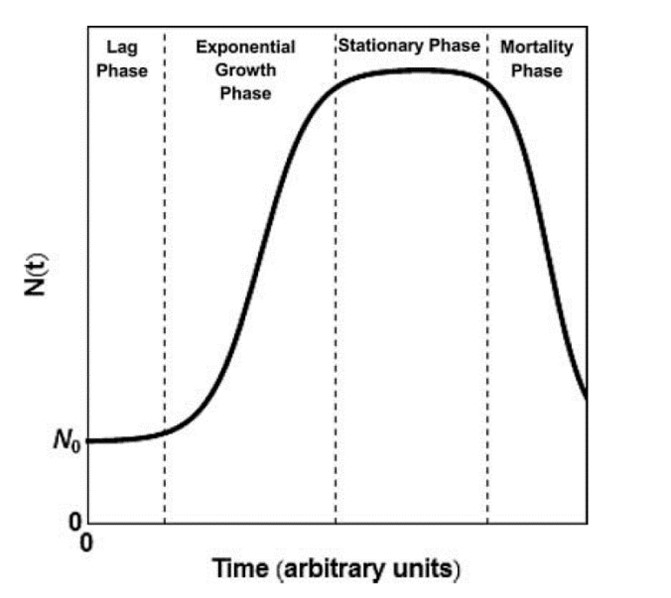
\includegraphics[width=0.6\textwidth]{figure1}
    \caption{Four distinguishable phases of bacterial growth in a closed habitat (Micha and Corradini, 2011) \cite{peleg2011microbial}}
    \label{figure1}
\end{figure}

Typically, there are four distinguishable phases of bacterial growth in a closed habitat as shown in Figure 1 above. They are “lag phase”, “exponential growth phase”, “stationary phase”, and “mortality phase” (McKellar and Lu, 2003) \cite{mckellar2003modeling}. But the “mortality phase” is ignored in most cases and only the first three phases are investigated in the food microbiology since foods will become harmful and inedible long before the "mortality phase" starts, and sometimes even before the "stationary phase" (Micha and Corradini, 2011) \cite{peleg2011microbial}.  

My objective of this study is to investigate how well different mathematical models, such as those based on population growth (mechanistic) theory vs. those based on phenomenological ones, fit the population growth data across the unique ID. The population growth data covers measurements of change in biomass or number of microbes cells over time and is collected through lab experiments throughout the world. Five different mathematical models can be applied to fit the population growth data using ordinary linear and non-linear least squares methods to find the ones which best fit the dataset. Additionally, the five mathematical models involve not only phenomenological quadratic and cubic polynomial models but also non-linear mechanistic models of population growth. After that, Akaike Information Criterion (AIC) and Bayesian information criterion (BIC) can be used to compare the models (Aho et al., 2014) \cite{aho2014model}.


\section{Methods}
\subsection{Data}
The population growth data was acquired through lab experiments around the world and includes measurements of change in biomass or the number of microbial cells over time. There are two main variables in the population growth data, PopBio (abundance) is the population or biomass measurement regarded as the response variable and Time is the measurement time regarded as the independent variable. Furthermore, a unique population growth curve can be identified by combining Species, Medium, Temperature, and Citation these four variables to create a new independent variable called ID. As a result, numerous subsets of the population growth data can be constructed according to each unique ID. After the data wrangling, no missing value was found in each column. There are some negative values in the Time column, and these values are very close to zero in general, so they are set to be zeros to make the data more realistic and meaningful. To obtain the log-transformed values, only the positive values of PopBio are saved since the independent variable of the logarithmic functional has to be greater than 0, which is followed by deriving a log-transformed PopBio column.


\subsection{Models}
To start with, two linear mathematical models were applied to fit each subset of the population growth data, namely the phenomenological quadratic and cubic polynomial models (Johnson et al., 2004) \cite{johnson2004model}. The equations (1) (2) of these two models are shown below respectively. 
\begin{equation}
y = ax^2 + bx + c
\end{equation}
\begin{equation}
y = ax^3 + bx^2 + cx + d
\end{equation}
The quadratic and cubic curve models can capture the curvature in data (Motulsky et al., 2004) \cite{motulsky2004fitting}. For non-linear mechanistic models, three different growth rate models were adopted to fit each subset in a similar way (Bolker et al., 2013) \cite{bolker2013strategies} . These mechanistic models are the logistic model, modified Gompertz model (Zwietering et. al., 1990) \cite{zwietering1990modeling}, and the Baranyi model (Baranyi, 1993) \cite{baranyi1993non}. A classical logistic equation (3) is displayed below. 
\begin{equation}
N_t = \frac{N_0Ke^{rt}}{K + N_0(e^{rt} - 1)}
\end{equation}
Here N\textsubscript{0} is the initial population size, N\textsubscript{t} is population size at time t, r is the maximum growth rate, and K is the maximum possible population abundance and is also called carrying capacity (Samraat Pawar, 2021) \cite{pawar}.  

However, there is a time lag in the microbial population growth. Before starting the exponential growth, bacteria need to spend some time adapting to the new environment or growth media and activating genes relating to intaking nutrition and metabolic processes (Rolfe et al., 2012) \cite{rolfe2012lag}. And the modified Gompertz model (Zwietering et. al., 1990) \cite{zwietering1990modeling} can be applied to capture the time lag when modeling the bacterial growth. The Gompertz equation (4) is a bit more complicated as shown below. 
\begin{equation}
log(N_t) = N_0 + (N_{max} - N_0)e^{-e^{r_{max}exp(1)\frac{t_{lag}-t}{(N_{max}-N_0)log(10)}+1}}
\end{equation}
Here t\textsubscript{lag} is the lag time before the exponential growth, r\textsubscript{max} is the maximum growth rate tangent to the inflection point, and log($\frac{N\textsubscript{max}}{N\textsubscript{0}}$) is the log ratio of the carrying capacity and the initial population size. In addition, the Gompertz model is in the log scale and designed to fit the log-transformed population growth data (Samraat Pawar, 2021) \cite{pawar}. 

Besides the Gompertz model, the Baranyi model (Baranyi, 1993) \cite{baranyi1993non} can also be used to describe the lag phase. The Baranyi equation (5) is displayed below. 
\begin{equation}
y(t) = y_0 + {\mu}{A(t)} - ln(1 + \frac{e^{{\mu}A(t)}-1}{e^C})
\end{equation}
\begin{equation}
A(t) = t + \frac{1}{\mu}ln(e^{{-\mu}{t}} + e^{{-\mu}{\lambda}} - e^{{-\mu}(t+{\lambda})}
\end{equation}
Here y is the population size in log scale at time t, y\textsubscript{0} is the initial population size in log scale, 
y\textsubscript{max} is the final population size in log scale, 
$\mu$ is the maximum growth rate, C is the difference between 
y\textsubscript{0} and y\textsubscript{max} in log scale, and 
$\lambda$ is the lag time before the exponential growth (Pla et al., 2015) \cite{pla2015comparison}. 


\subsection{Model fitting}
The linear quadratic and cubic polynomial models can be easily applied to fit the data using the lm function in R. The goodness-of-fit is evaluated by the summary function and the coefficients of models can be acquired subsequently.  

For the non-linear mechanistic models, several starting parameters need to be defined previously. To start with, a linear model can be used to fit the data. And the slope of the Time variable can be adopted to be the starting value of the maximum growth rate. For the logistic model, the starting values of N\textsubscript{0} and K are assigned to be the lowest population size and highest population size respectively.  

For the modified Gompertz model and Baranyi model, the starting values of initial population size and final population size are set to be the lowest population size and highest one both in the log scale respectively. To find the last time point of the lag phase, the whole dataset is sliced into the first third of it, and the lag time is the time point where the second-order derivative of the differentials is maximal. Then a non-linear least squares (NLLS) model fitting function called nlsLM in R can be used to fit each model using the starting values derived above, followed by obtaining the model summary. Moreover, the try function is applied in the non-linear least squares model fitting to capture errors when the fitting does not converge. 
\subsection{Plotting and analysis}
To observe the goodness-of-fit of each model, every unique population growth curve is plotted with these five models overlaid. In addition, the main coefficients of each model as well as AIC, BIC, and R squared values of model fitting are separately saved in csv files for subsequent review and analysis. For the subsets of the population growth data, the number of times that the AIC or BIC value of each model is the lowest in the same subset can be acquired to find the models which best fit the dataset. 
\subsection{Computing tools}
For this mini-project, R is the main scripting language for data preparation, model fitting, and final plotting and analysis, since it is more convenient and coherent for me to use the same language. And I also use bash to compile the LaTeX report and run the whole project. In R, nls.lm package is necessary because the nlsLM function is used, and ggplot2 is loaded to generate beautiful figures for plotting.  
\section{Results}
As outlined in the introduction, in order to find the models which best fit the dataset, five different mathematical models are applied to fit the population growth data across the unique ID. After running the model fitting script, several csv files are generated to display the coefficients of each model as well as the corresponding AIC, BIC, and R squared values. As the phenomenological models, quadratic and cubic polynomial models fit the data linearly. For the mechanistic ones, the modified Gompertz model fitting succeeds 208 times and fails 77 times and the Baranyi model succeeds 139 times and fails 146 times. However, the logistic model fits each data subset successfully.

\begin{figure}[H]
    \centering
    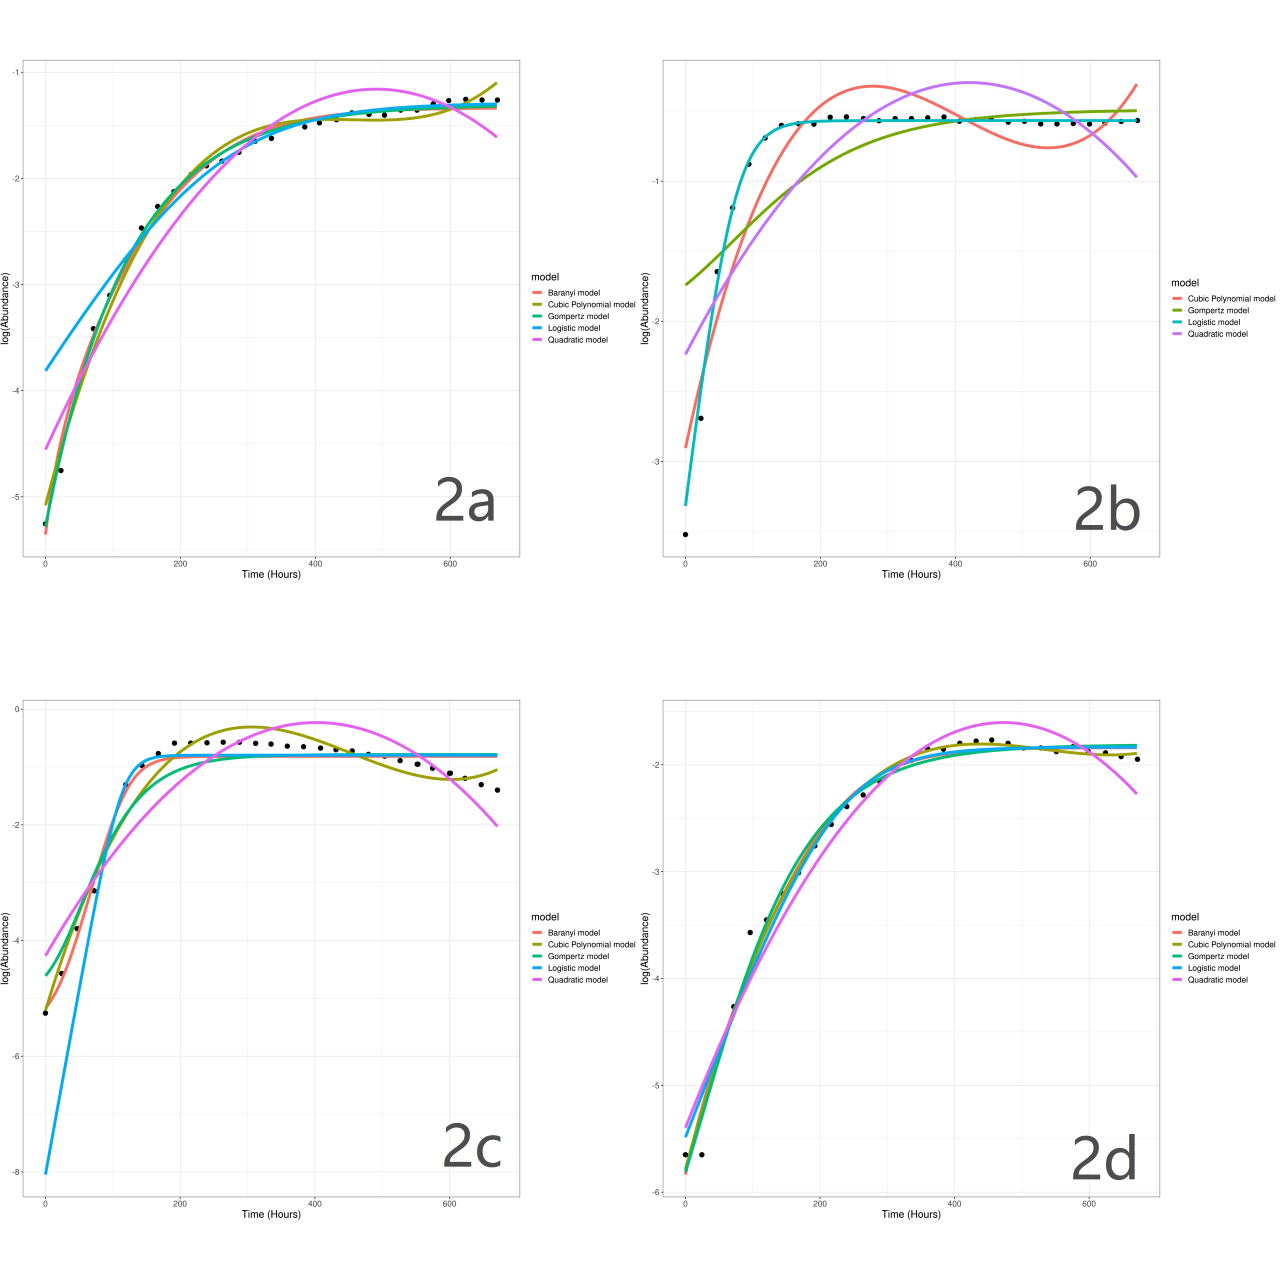
\includegraphics[width=\textwidth]{figure2}
    \caption{Four distinct plots of different data subsets}
    \label{figure2}
\end{figure}

After running the plotting and analysis script, 285 population growth scatter plots are created with the mathematical model curves overlaid. Four distinct plots of different data subsets are displayed in Figure 2 above. As shown in figure 2a, the quadratic model fits the data imprecisely and only a few data points fall on the curve. This model roughly describes the change in biomass over time, but it captures the “mortality phase” of population growth after the carrying capacity has been reached. The cubic polynomial model fits the data more accurately than the quadratic one and the cubic curve even fits the data points well at the lower end. However, in contrast to the quadratic model, the cubic curve goes up unexpectedly after the “stationary phase” of population growth is reached. For the non-linear mechanistic models, the logistic model visibly deviates from the data at the initial stage, but it highly fits the remaining part of the data. And it can be seen that the Gompertz model and Baranyi model both fit the data perfectly and the curves of the three mechanistic models overlap nicely at the “stationary phase”.  

As shown in figure 2b, similarly, the quadratic model fits the data roughly. It seems that the quadratic curve only passes through two data points, and it has little to do with the variation in the data. As expected, the quadratic curve also captures the “mortality phase” of population growth in this case. However, the cubic polynomial model fits the data poorly at this time and the cubic curve also rises after the “stationary phase”. For the mechanistic models, the Baranyi curve fails to show up since there might have some errors in the model fitting process. It can be observed that the Gompertz model also fits the data poorly and it diverges from the data on the whole. Fortunately, the logistic model fits this data subset excellently and nearly all the data points fall on the logistic curve. 

As indicated in figure 2c, both the quadratic model and cubic model can catch the decrease in the population size after the maximum value is reached and they can delineate the trends in the data sketchily. For the mechanistic ones, the logistic model obviously deviates from the data in the beginning. While the Baranyi model slightly diverges from the data after finishing the “exponential growth phase” and the Gompertz model fails to fit the data well in general. Additionally, these three non-linear models overlap together in the final stage, deviating from the declining data points.  

As indicated in figure 2d, similarly, the quadratic model roughly depicts the changes in data and captures the decrease in the data points after the carrying capacity has been attained. In this case, the cubic model fits the data nicely and even approaches the data at the lower end. For the mechanistic models, the logistic model again diverges from the data at the early stage but fits the remaining section well. The Gompertz model and Baranyi model have very similar effects on data fitting for this subset. These three non-linear models are highly overlapped after the “exponential growth phase” has finished and unable to describe the downward trajectory. 

\begin{figure}[H]
    \centering
    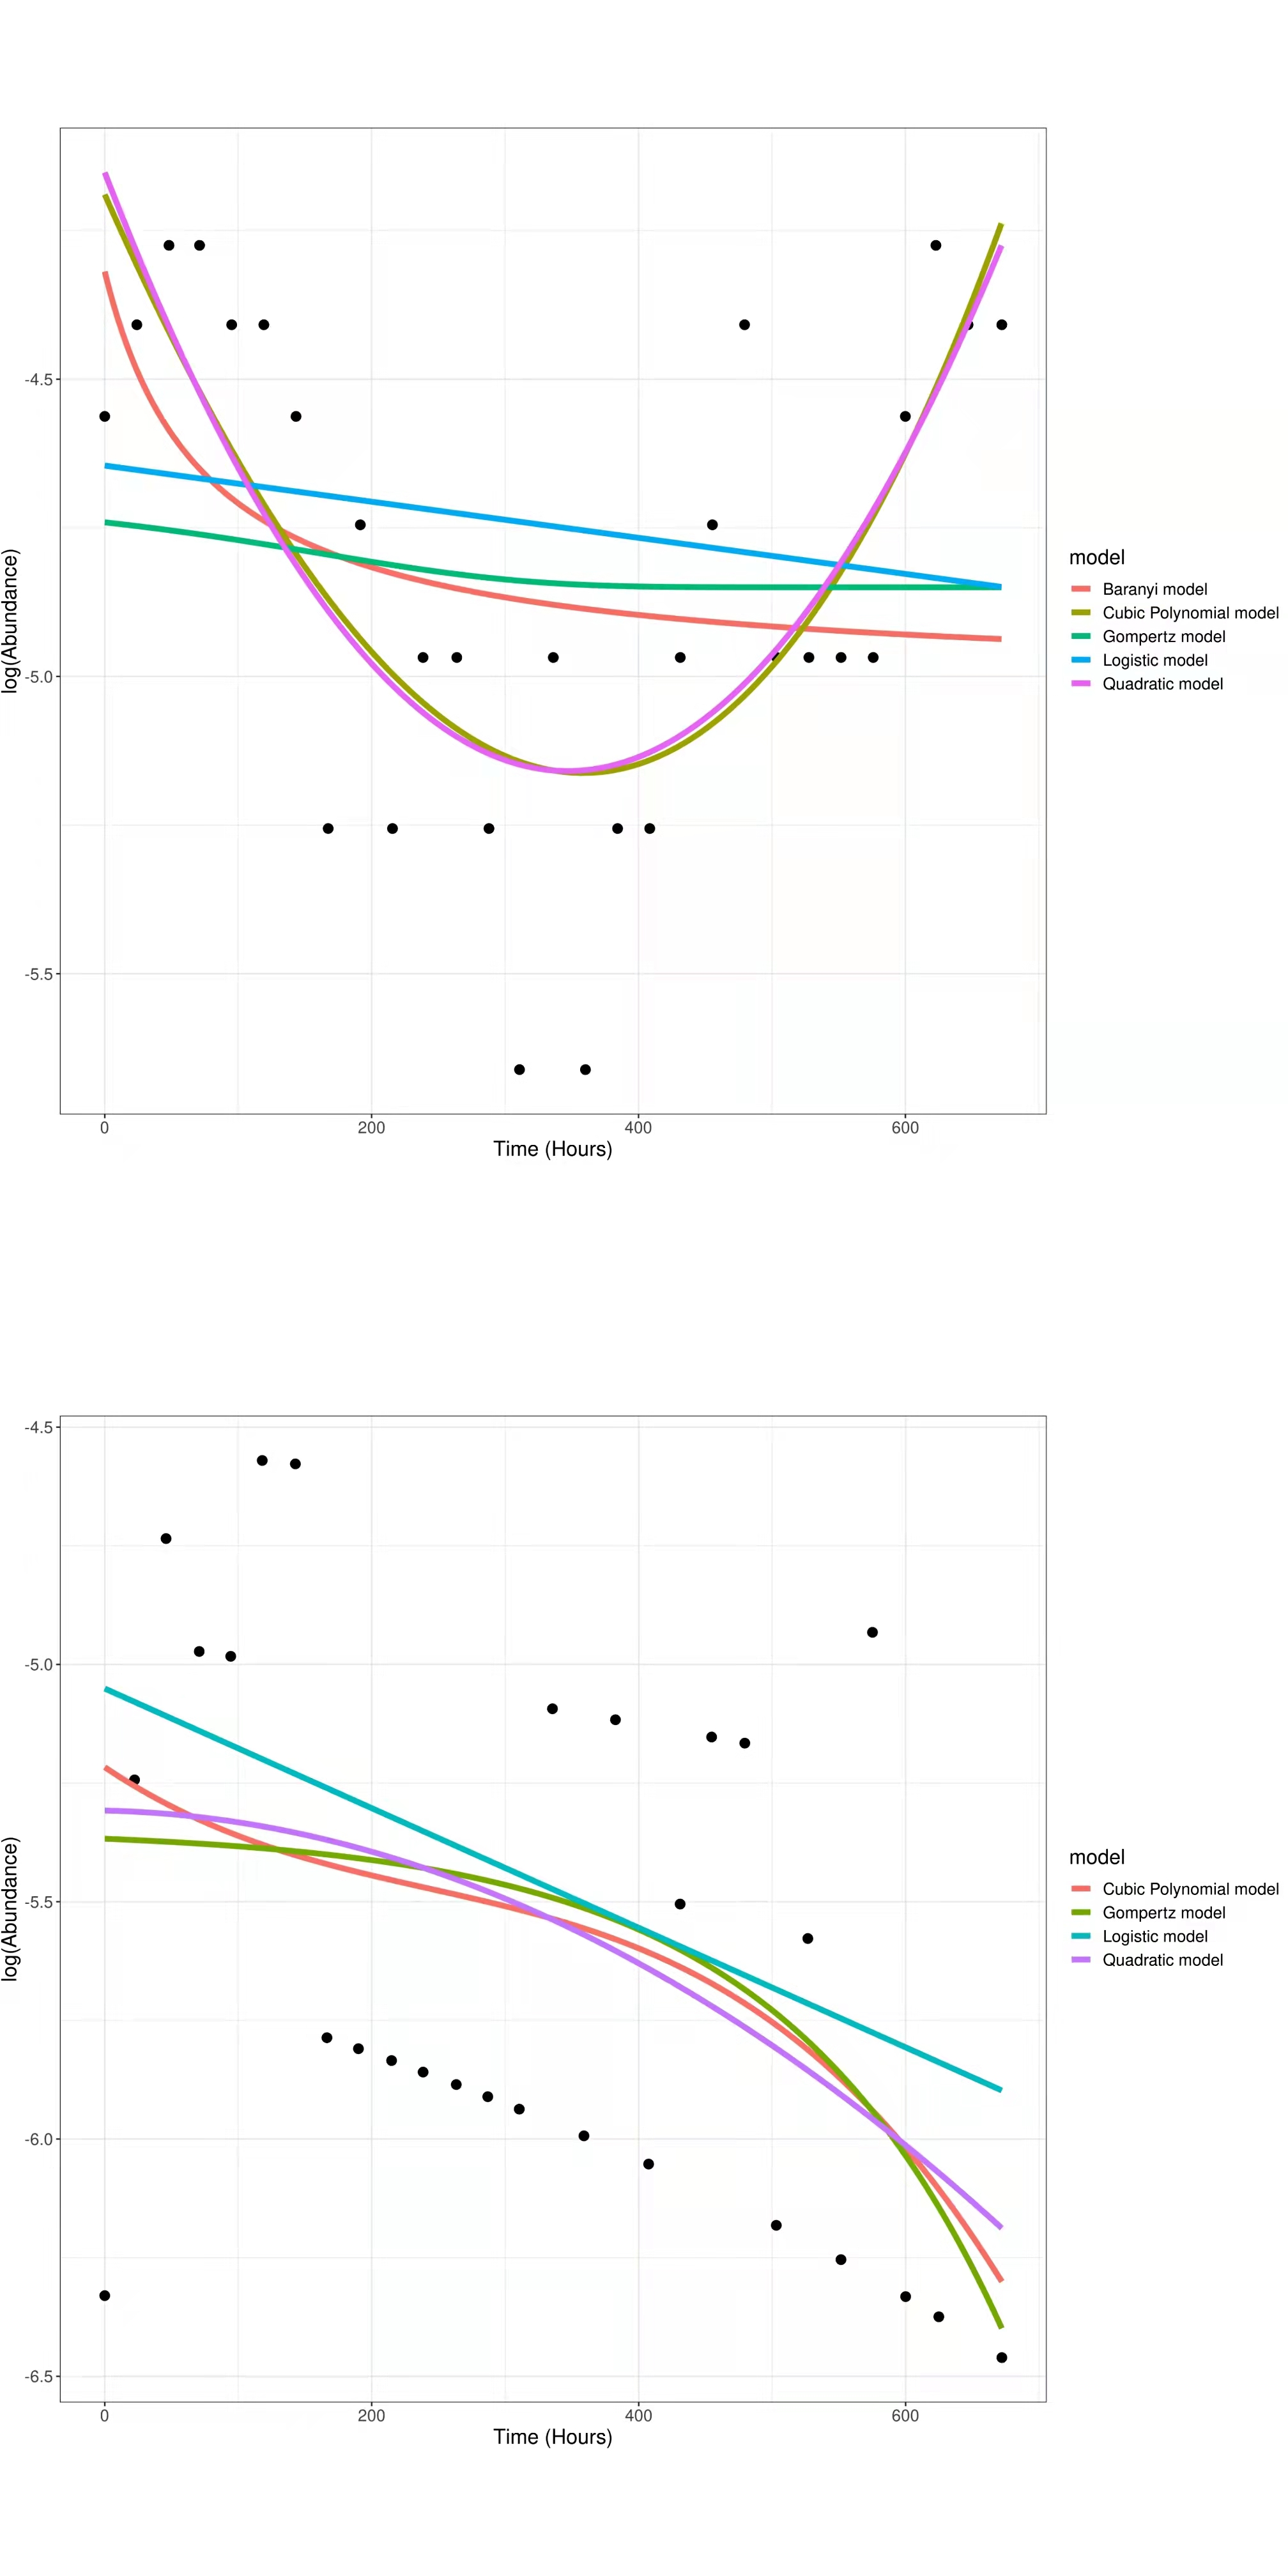
\includegraphics[width=0.6\textwidth]{figure3}
    \caption{Subsets with scattered and irregular data points}
    \label{figure3}
\end{figure}

However, as displayed in figure 3, data points of some subsets are extremely scattered and irregular, and no model can fit these data well. And it is apparent in Figure 4 that the logistic model completely fails to fit the data at the lag phase, while the rest of the models can delineate the data well before the “exponential growth phase” is reached. 

\begin{figure}[H]
    \centering
    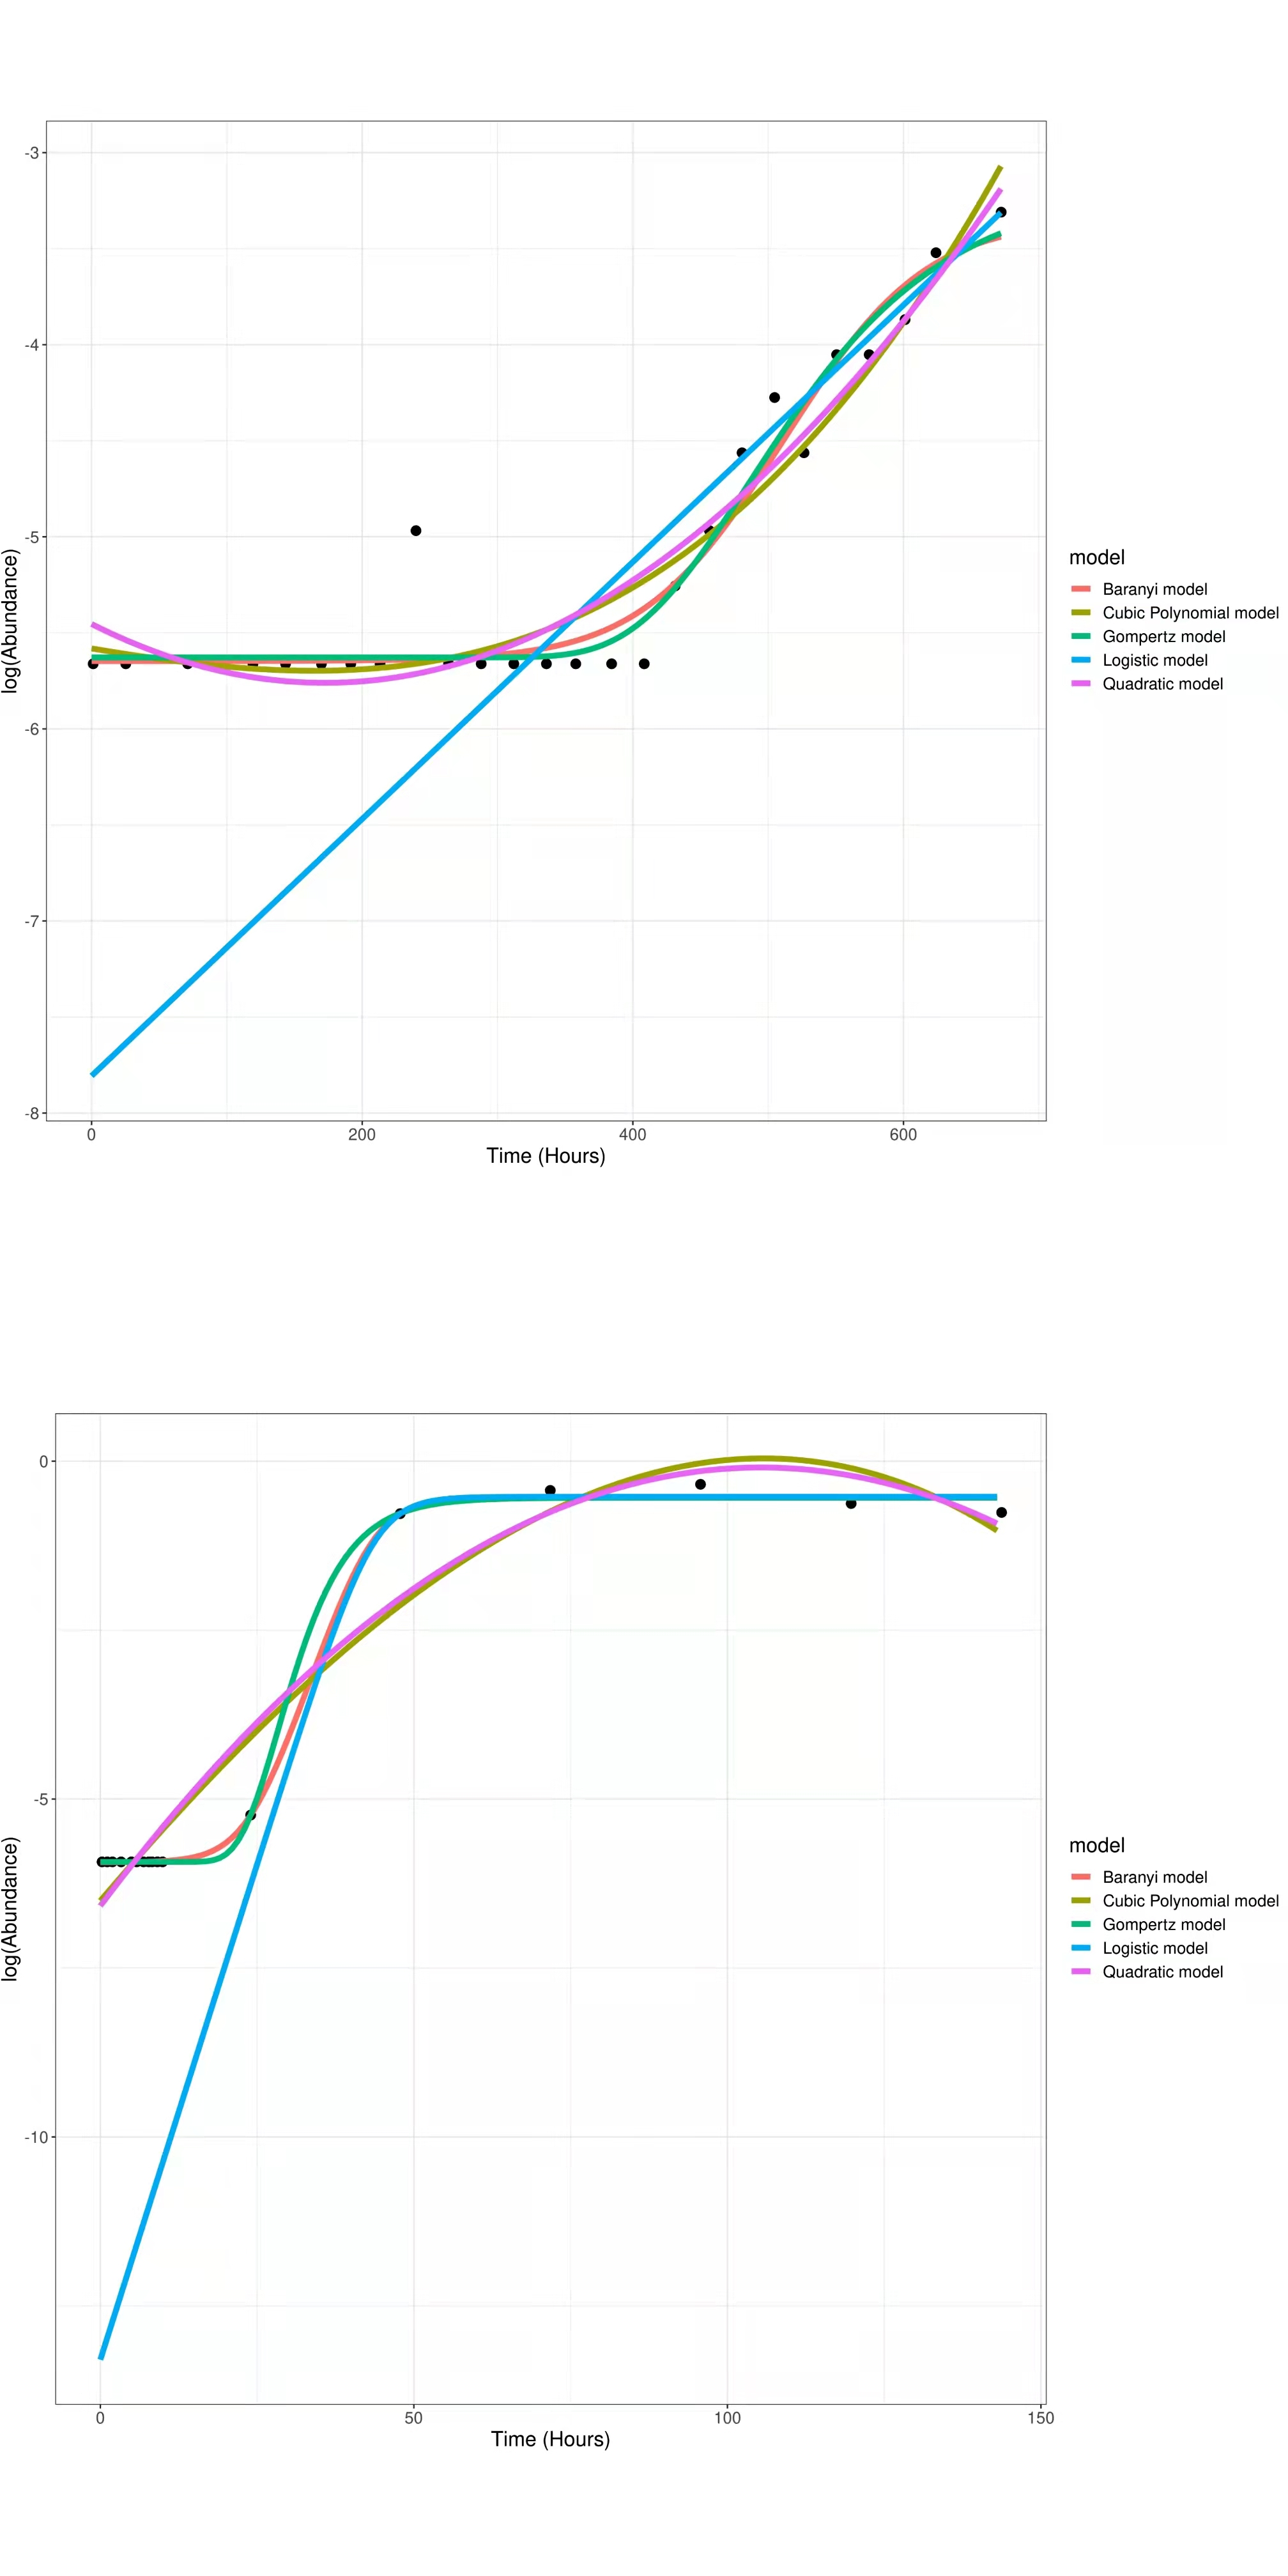
\includegraphics[width=0.6\textwidth]{figure4}
    \caption{Subsets with distinctive lag phases}
    \label{figure4}
\end{figure}

\begin{figure}[H]
    \centering
    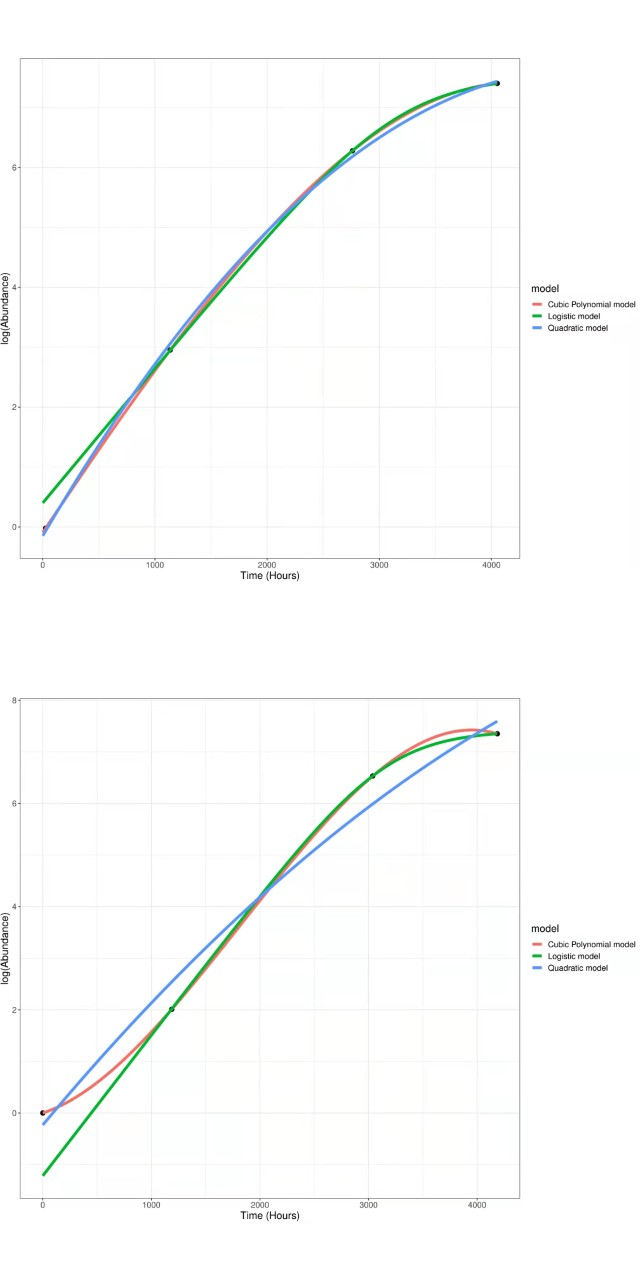
\includegraphics[width=0.6\textwidth]{figure5}
    \caption{Subsets with only a few data points}
    \label{figure5}
\end{figure}
Especially, what stands out in Figure 5 is that these subsets have only a few data points, and the number of microbial cells increases nearly linearly over time. Therefore, the quadratic and cubic polynomial models fit the data really well, the AIC and BIC values of the cubic models are calculated as negative infinity. While the Gompertz and Baranyi curves do not appear because the model fitting doesn’t converge.  
\begin{figure}[H]
    \centering
    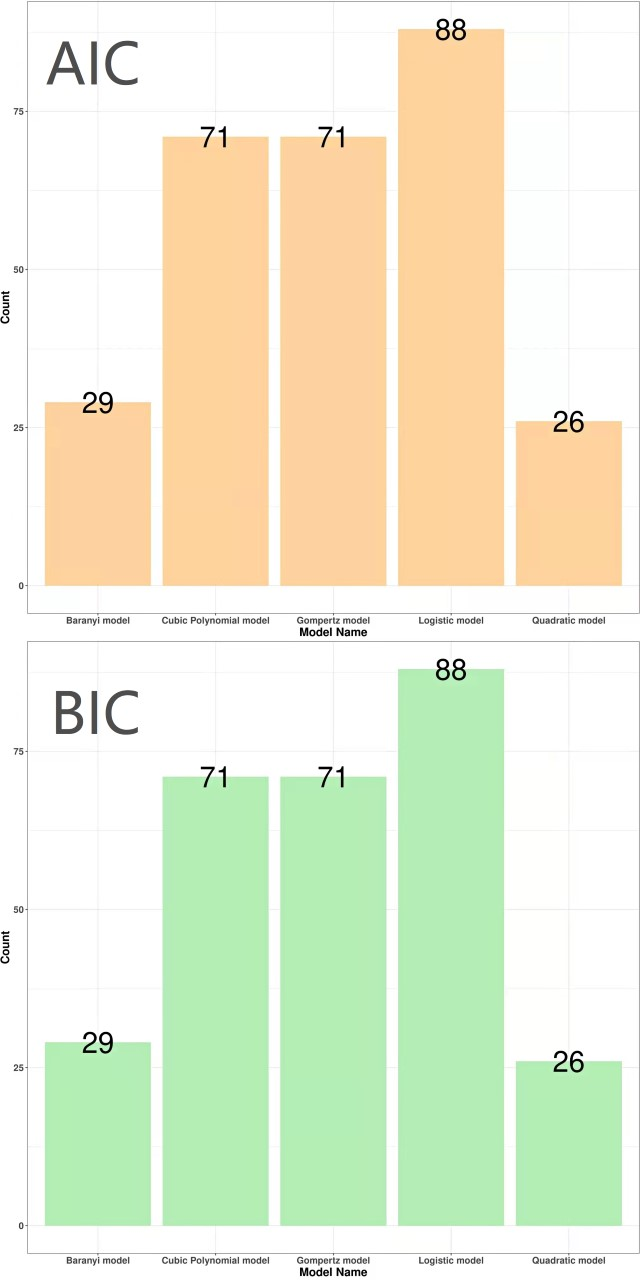
\includegraphics[width=0.6\textwidth]{figure6}
    \caption{Number of cases with the smallest AIC/BIC value in each model}
    \label{figure6}
\end{figure}
As for comparing and selecting models, the AIC and BIC values of these five mathematical models are calculated for all the 285 subsets. Interestingly, it can be observed that the number of cases when the AIC and BIC values of the logistic model are the lowest among the five models is 88. And the count of logistic model with the minimum AIC and BIC values is the largest. As demonstrated in Figure 6, the quadratic model has the lowest AIC and BIC values 26 times, the cubic polynomial model has the lowest AIC and BIC values 71 times, the Gompertz model has the lowest AIC and BIC values 71 times, and the Baranyi model has the lowest AIC and BIC values 29 times. 

\section{Discussion}
As stated above, five different mathematical models are adopted to fit the population growth data throughout the unique ID using ordinary linear and non-linear least squares methods to determine the models that best fit the dataset. One interesting finding is that although the quadratic model fits the data roughly, it can capture the “mortality phase” of population growth after the carrying capacity has been reached in most subsets. There are several cases of cubic polynomial model fitting for the population growth data. This model fits the data nicely in some subsets but poorly in others. In some cases, its curve goes up unexpectedly after the “stationary phase” is reached but in other cases, it captures the decrease in the population size after the maximum value is achieved. 

For the mechanistic ones, the logistic model usually obviously diverges from the data at the “lag phase” but fits the remaining section pretty well in most subsets. The Gompertz model fitting can successfully converge in the majority of subsets. It fits the data perfectly in some cases but poorly in others, deviating from the data on the whole. And the Baranyi model fitting fails to converge in more than half of the subsets. But its curve fits the data excellently in general as long as the model fitting converges successfully. Furthermore, in most cases, the three non-linear models overlap together after the “stationary phase” has reached and are unable to describe the downward trajectory of the data. One noticeable finding is that if subsets have only a few data points, the cubic model fits the data remarkably. 

Moreover, because the lower AIC or BIC, the better, the results of AIC and BIC values surprisingly suggest that the logistic model best fits the population growth data on the whole, while the quadratic model is the most inaccurate one to fit the data. The cubic polynomial model and modified Gompertz model generally fit the population growth data well at similar levels. The former is a phenomenological model and the latter, as a mechanistic model, fails to fit the data 77 times out of 285 subsets. Meanwhile, the Baranyi model poorly fits the whole dataset since the model fitting is unable to converge 146 times. And Baranyi model emerges as a winner 29 times out of the 139 successful convergences. 

Unfortunately, the findings above are contrary to previous studies (Zwietering et al., 1990) \cite{zwietering1990modeling} which have suggested that the Gompertz model fitted all growth curves better than the linear, quadratic, \textit{t}th-power, logistic, and exponential models and was considered the best model to delineate the growth data in most cases. A possible explanation for this may be that the starting values of the primary parameters are not set to be quite appropriate by using the non-linear least squares method, leading to the inaccurate Gompertz models. In addition, it has been suggested that the Baranyi model was more advantageous than the Gompertz model in terms of goodness-of-fit at higher growth rates (Baranyi et al., 1993) \cite{baranyi1993non}. And López et al. (2004) \cite{lopez2004statistical} also reported that the Baranyi model showed a remarkably outstanding ability to fit the microbial growth data than the Gompertz model. The findings above again seem to be inconsistent with the previous research. This discrepancy may be explained by the facts that the starting values of the Baranyi model parameters deviate from the proper ones using the non-linear least squares method and the population growth data itself contains a large number of problematic and disorganized subsets. Although the findings above do not support the previous studies, they can still provide new insights into the phenomenological and mechanistic model fitting for the population growth data. 

The findings are not very encouraging since they disagree with the previous research. The inconsistency may be due to the inaccurate starting values of the important parameters in the mechanistic models, problematic and scattered values in the population growth dataset, and the single criterion (AIC/BIC) for model comparison and selection.  

Therefore, further research can be undertaken to set the starting values in the mechanistic models more precisely such as using the rolling regression, remove the low-quality values in the dataset, and adopt more complicated methods to compare and select models such as Akaike Weights and Likelihood-Ratio test. 

\section{Conclusion}
To sum up, five different mathematical models are applied to fit the population growth data using ordinary linear and non-linear least squares methods to find the ones which best fit the dataset. The count of logistic model with the minimum AIC and BIC values is the largest, which indicates that the logistic model best fits the population growth data on the whole. And the logistic curve usually visibly diverges from the data at the “lag phase” but fits the remaining section pretty well in most subsets. The quadratic model is the most inaccurate one to fit the data, but it can capture the “mortality phase” of population growth after the carrying capacity has been reached in most cases. The cubic polynomial model and modified Gompertz model generally fit the population growth data well at similar levels. Meanwhile, the Baranyi model poorly fits the whole dataset since the model fitting fails to converge in more than half of the subsets. But its curve fits the data nicely in general as long as the model fitting converges successfully. Although the findings are contrary to the previous research, they can still provide new insights into the phenomenological and mechanistic model fitting for the population growth dataset using ordinary linear and non-linear least squares methods. 



\bibliographystyle{plain}
\bibliography{citation}
\end{document}
